% This is the Reed College LaTeX thesis template. Most of the work
% for the document class was done by Sam Noble (SN), as well as this
% template. Later comments etc. by Ben Salzberg (BTS). Additional
% restructuring and APA support by Jess Youngberg (JY).
% Your comments and suggestions are more than welcome; please email
% them to cus@reed.edu
%
% See http://web.reed.edu/cis/help/latex.html for help. There are a
% great bunch of help pages there, with notes on
% getting started, bibtex, etc. Go there and read it if you're not
% already familiar with LaTeX.
%
% Any line that starts with a percent symbol is a comment.
% They won't show up in the document, and are useful for notes
% to yourself and explaining commands.
% Commenting also removes a line from the document;
% very handy for troubleshooting problems. -BTS

% As far as I know, this follows the requirements laid out in
% the 2002-2003 Senior Handbook. Ask a librarian to check the
% document before binding. -SN

%%
%% Preamble
%%
% \documentclass{<something>} must begin each LaTeX document
\documentclass[12pt,twoside]{reedthesis}
% Packages are extensions to the basic LaTeX functions. Whatever you
% want to typeset, there is probably a package out there for it.
% Chemistry (chemtex), screenplays, you name it.
% Check out CTAN to see: http://www.ctan.org/
%%
\usepackage{graphicx,latexsym}
\usepackage{amsmath}
\usepackage{amssymb,amsthm}
\usepackage{longtable,booktabs,setspace}
\usepackage{chemarr} %% Useful for one reaction arrow, useless if you're not a chem major
\usepackage[hyphens]{url}
% Added by CII
\usepackage{hyperref}
\usepackage{lmodern}
\usepackage{float}
\floatplacement{figure}{H}
% End of CII addition
\usepackage{rotating}

% Next line commented out by CII
%%% \usepackage{natbib}
% Comment out the natbib line above and uncomment the following two lines to use the new
% biblatex-chicago style, for Chicago A. Also make some changes at the end where the
% bibliography is included.
%\usepackage{biblatex-chicago}
%\bibliography{thesis}


% Added by CII (Thanks, Hadley!)
% Use ref for internal links
\renewcommand{\hyperref}[2][???]{\autoref{#1}}
\def\chapterautorefname{Chapter}
\def\sectionautorefname{Section}
\def\subsectionautorefname{Subsection}
% End of CII addition

% Added by CII
\usepackage{caption}
\captionsetup{width=5in}
% End of CII addition

% \usepackage{times} % other fonts are available like times, bookman, charter, palatino

% Syntax highlighting #22
  \usepackage{color}
  \usepackage{fancyvrb}
  \newcommand{\VerbBar}{|}
  \newcommand{\VERB}{\Verb[commandchars=\\\{\}]}
  \DefineVerbatimEnvironment{Highlighting}{Verbatim}{commandchars=\\\{\}}
  % Add ',fontsize=\small' for more characters per line
  \usepackage{framed}
  \definecolor{shadecolor}{RGB}{248,248,248}
  \newenvironment{Shaded}{\begin{snugshade}}{\end{snugshade}}
  \newcommand{\KeywordTok}[1]{\textcolor[rgb]{0.13,0.29,0.53}{\textbf{{#1}}}}
  \newcommand{\DataTypeTok}[1]{\textcolor[rgb]{0.13,0.29,0.53}{{#1}}}
  \newcommand{\DecValTok}[1]{\textcolor[rgb]{0.00,0.00,0.81}{{#1}}}
  \newcommand{\BaseNTok}[1]{\textcolor[rgb]{0.00,0.00,0.81}{{#1}}}
  \newcommand{\FloatTok}[1]{\textcolor[rgb]{0.00,0.00,0.81}{{#1}}}
  \newcommand{\ConstantTok}[1]{\textcolor[rgb]{0.00,0.00,0.00}{{#1}}}
  \newcommand{\CharTok}[1]{\textcolor[rgb]{0.31,0.60,0.02}{{#1}}}
  \newcommand{\SpecialCharTok}[1]{\textcolor[rgb]{0.00,0.00,0.00}{{#1}}}
  \newcommand{\StringTok}[1]{\textcolor[rgb]{0.31,0.60,0.02}{{#1}}}
  \newcommand{\VerbatimStringTok}[1]{\textcolor[rgb]{0.31,0.60,0.02}{{#1}}}
  \newcommand{\SpecialStringTok}[1]{\textcolor[rgb]{0.31,0.60,0.02}{{#1}}}
  \newcommand{\ImportTok}[1]{{#1}}
  \newcommand{\CommentTok}[1]{\textcolor[rgb]{0.56,0.35,0.01}{\textit{{#1}}}}
  \newcommand{\DocumentationTok}[1]{\textcolor[rgb]{0.56,0.35,0.01}{\textbf{\textit{{#1}}}}}
  \newcommand{\AnnotationTok}[1]{\textcolor[rgb]{0.56,0.35,0.01}{\textbf{\textit{{#1}}}}}
  \newcommand{\CommentVarTok}[1]{\textcolor[rgb]{0.56,0.35,0.01}{\textbf{\textit{{#1}}}}}
  \newcommand{\OtherTok}[1]{\textcolor[rgb]{0.56,0.35,0.01}{{#1}}}
  \newcommand{\FunctionTok}[1]{\textcolor[rgb]{0.00,0.00,0.00}{{#1}}}
  \newcommand{\VariableTok}[1]{\textcolor[rgb]{0.00,0.00,0.00}{{#1}}}
  \newcommand{\ControlFlowTok}[1]{\textcolor[rgb]{0.13,0.29,0.53}{\textbf{{#1}}}}
  \newcommand{\OperatorTok}[1]{\textcolor[rgb]{0.81,0.36,0.00}{\textbf{{#1}}}}
  \newcommand{\BuiltInTok}[1]{{#1}}
  \newcommand{\ExtensionTok}[1]{{#1}}
  \newcommand{\PreprocessorTok}[1]{\textcolor[rgb]{0.56,0.35,0.01}{\textit{{#1}}}}
  \newcommand{\AttributeTok}[1]{\textcolor[rgb]{0.77,0.63,0.00}{{#1}}}
  \newcommand{\RegionMarkerTok}[1]{{#1}}
  \newcommand{\InformationTok}[1]{\textcolor[rgb]{0.56,0.35,0.01}{\textbf{\textit{{#1}}}}}
  \newcommand{\WarningTok}[1]{\textcolor[rgb]{0.56,0.35,0.01}{\textbf{\textit{{#1}}}}}
  \newcommand{\AlertTok}[1]{\textcolor[rgb]{0.94,0.16,0.16}{{#1}}}
  \newcommand{\ErrorTok}[1]{\textcolor[rgb]{0.64,0.00,0.00}{\textbf{{#1}}}}
  \newcommand{\NormalTok}[1]{{#1}}

% To pass between YAML and LaTeX the dollar signs are added by CII
\title{Forecasting Constituents of the MSCI Minimum Volatility Index Through
Logistic Regression}
\author{John A. Gilheany}
% The month and year that you submit your FINAL draft TO THE LIBRARY (May or December)
\date{November 6, 2017}
\division{Statistics}
\advisor{Professor Michael Parzen}
\institution{Harvard College}
\degree{Bachelor of Arts in Statistics (Honors)}
%If you have two advisors for some reason, you can use the following
% Uncommented out by CII
\altadvisor{David Kane}
% End of CII addition

%%% Remember to use the correct department!
\department{Statistics}
% if you're writing a thesis in an interdisciplinary major,
% uncomment the line below and change the text as appropriate.
% check the Senior Handbook if unsure.
%\thedivisionof{The Established Interdisciplinary Committee for}
% if you want the approval page to say "Approved for the Committee",
% uncomment the next line
%\approvedforthe{Committee}

% Added by CII
%%% Copied from knitr
%% maxwidth is the original width if it's less than linewidth
%% otherwise use linewidth (to make sure the graphics do not exceed the margin)
\makeatletter
\def\maxwidth{ %
  \ifdim\Gin@nat@width>\linewidth
    \linewidth
  \else
    \Gin@nat@width
  \fi
}
\makeatother

\renewcommand{\contentsname}{Table of Contents}
% End of CII addition

\setlength{\parskip}{0pt}

% Added by CII

\providecommand{\tightlist}{%
  \setlength{\itemsep}{0pt}\setlength{\parskip}{0pt}}

\Acknowledgements{
I want to thank Prof.~Parzen and David Kane for all of their help.
}

\Dedication{

}

\Preface{
This thesis explores a way of predicting index constituents using
logistic regression.
}

\Abstract{
The low-risk anomaly has created opportunities for arbitrage in the
financial markets. As Baker et al. discuss in ``Benchmarks as Limits to
Arbitrage: Understanding the Low-Volatility Anomaly,'' low-volatility
and low-beta portfolios outperform and high-volatility and high-beta
portfolios by a factor of several times due to benchmarking and
lottery-preferences. The iShares MSCI USA Minimum Volatility (USMV) is
an ETF tracking a minimum volatility index that was used to find data
and will be used for trading arbitrage. Frazzini et al. discuss
arbitrage opportunities by quantitative focused funds like AQR in
``Betting Against Beta'', and this thesis explores a more advanced type
of index front-running as a potential arbitrage opportunity. Data was
collected from USMV from its inception in October 2011, and from EUSA,
the parent ETF of USMV, from the same period until December 2016.
52-week trailing beta, 52-week trailing volatility, lagged price/book,
and current index membership were calculated, and a regression model was
run to quantify the relationship between current index membership and
these four variables. In the model, a probabilities of index membership
were calculated and an optimal cutoff was calculated to which the model
would be 95\% accurate of its findings of a stock to be in or out of
USMV, given the historical data. Backtesting with prior data showed with
a model accuracy of 95\%, arbitrage opportunities of X\% could be
collected after each rebalancing.
}

% End of CII addition
%%
%% End Preamble
%%
%

\usepackage{amsthm}
\newtheorem{theorem}{Theorem}[chapter]
\newtheorem{lemma}{Lemma}[chapter]
\theoremstyle{definition}
\newtheorem{definition}{Definition}[chapter]
\newtheorem{corollary}{Corollary}[chapter]
\newtheorem{proposition}{Proposition}[chapter]
\theoremstyle{definition}
\newtheorem{example}{Example}[chapter]
\theoremstyle{definition}
\newtheorem{exercise}{Exercise}[chapter]
\theoremstyle{remark}
\newtheorem*{remark}{Remark}
\newtheorem*{solution}{Solution}
\begin{document}

% Everything below added by CII
  \maketitle

\frontmatter % this stuff will be roman-numbered
\pagestyle{empty} % this removes page numbers from the frontmatter
  \begin{acknowledgements}
    I want to thank Prof.~Parzen and David Kane for all of their help.
  \end{acknowledgements}
  \begin{preface}
    This thesis explores a way of predicting index constituents using
    logistic regression.
  \end{preface}
  \hypersetup{linkcolor=black}
  \setcounter{tocdepth}{2}
  \tableofcontents

  \listoftables

  \listoffigures
  \begin{abstract}
    The low-risk anomaly has created opportunities for arbitrage in the
    financial markets. As Baker et al. discuss in ``Benchmarks as Limits to
    Arbitrage: Understanding the Low-Volatility Anomaly,'' low-volatility
    and low-beta portfolios outperform and high-volatility and high-beta
    portfolios by a factor of several times due to benchmarking and
    lottery-preferences. The iShares MSCI USA Minimum Volatility (USMV) is
    an ETF tracking a minimum volatility index that was used to find data
    and will be used for trading arbitrage. Frazzini et al. discuss
    arbitrage opportunities by quantitative focused funds like AQR in
    ``Betting Against Beta'', and this thesis explores a more advanced type
    of index front-running as a potential arbitrage opportunity. Data was
    collected from USMV from its inception in October 2011, and from EUSA,
    the parent ETF of USMV, from the same period until December 2016.
    52-week trailing beta, 52-week trailing volatility, lagged price/book,
    and current index membership were calculated, and a regression model was
    run to quantify the relationship between current index membership and
    these four variables. In the model, a probabilities of index membership
    were calculated and an optimal cutoff was calculated to which the model
    would be 95\% accurate of its findings of a stock to be in or out of
    USMV, given the historical data. Backtesting with prior data showed with
    a model accuracy of 95\%, arbitrage opportunities of X\% could be
    collected after each rebalancing.
  \end{abstract}

\mainmatter % here the regular arabic numbering starts
\pagestyle{fancyplain} % turns page numbering back on

\chapter{thesisdown::thesis\_gitbook:
default}\label{thesisdownthesis_gitbook-default}

Placeholder

\chapter{Introduction}\label{introduction}

Placeholder

\section{Background}\label{background}

\subsection{Exchange Traded Funds
(ETFs)}\label{exchange-traded-funds-etfs}

\subsection{iShares MSCI Min Vol USA
ETF}\label{ishares-msci-min-vol-usa-etf}

\subsection{Purpose}\label{purpose}

\subsection{Logistic Regression Model}\label{logistic-regression-model}

\section{Literature Review}\label{literature-review}

\subsection{Overview of the Low-Risk
Anomaly}\label{overview-of-the-low-risk-anomaly}

\subsection{Evidence of the Low-Risk
Anomaly}\label{evidence-of-the-low-risk-anomaly}

\subsubsection{Measures of Risk}\label{measures-of-risk}

\subsubsection{1929-2015}\label{section}

\subsubsection{1968-2008}\label{section-1}

\subsubsection{Critique of the Capital Asset Pricing
Model}\label{critique-of-the-capital-asset-pricing-model}

\subsection{Possible Explanations for the Low-Risk
Anomaly}\label{possible-explanations-for-the-low-risk-anomaly}

\subsubsection{Compounding}\label{compounding}

\subsubsection{Benchmarking}\label{benchmarking}

\subsubsection{Single-Period Returns}\label{single-period-returns}

\subsubsection{Psychological and Behavioral
Factors}\label{psychological-and-behavioral-factors}

\subsubsection{Profitability and Value}\label{profitability-and-value}

\subsection{Further Decomposition of the Low-Risk Anomaly into Micro and
Macro
Effects}\label{further-decomposition-of-the-low-risk-anomaly-into-micro-and-macro-effects}

\subsection{Real-World Applications of the Low-Risk
Anomaly}\label{real-world-applications-of-the-low-risk-anomaly}

\subsubsection{Betting Against Beta
(BaB)}\label{betting-against-beta-bab}

\subsubsection{Betting Against
Correlation}\label{betting-against-correlation}

\subsubsection{Stock Price Response to Index
Rebalancing}\label{stock-price-response-to-index-rebalancing}

\chapter{Data Gathering Process}\label{data-gathering-process}

\section{Data Aggregation}\label{data-aggregation}

Data was collected for the iShares MSCI USA Equal Weighted ETF (EUSA),
which tracks the parent index of the minimum volatiltiy index, and
iShares Edge MSCI Min Vol USA ETF (USMV), which tracks the minimum
volatility index, from Oct 31, 2011 to December 31, 2016 (BlackRock,
2017). The iShares data contained this information for the two ETFs of
interest for each constituent on the last trading day of every month.
This included characteristics of each stock, such as: ticker, company
name, asset class, weight of the stock relative to the entire index,
price per share, number of shares, market value of the position,
notional value of the position, sector, sedol number, isin number,
exchange that the stock is listed on, and the month end date for the
data. Each month-end dataset was individually downloaded, then
aggregated to create the two separate raw data sets - one for EUSA and
one for USMV. The data was then cleaned.

\section{Data Cleaning}\label{data-cleaning}

After having a quick overview of the data, there were many issues with
each respective dataset that needed to be fixed before the analysis
could occur. Since USMV is a subset of EUSA, the issues were very
similar, and those that existed in USMV, generally existed in USMV as
well. The issues could be broken down into 3 main types: erroneous
listed stock exchanges, problematic listed tickers, and price
discrepancies due to issues like stock splits. Moreover, cash and cash
related assets were removed from the data, as this dissertation focuses
only on the stocks.

\subsection{Non-US Exchanges}\label{non-us-exchanges}

Looking at the unique exchanges of the data, it was observed that there
were several foreign exchanges like the Swiss Exchange and the Mexican
Stock Exchange. For example, in the EUSA data set, there were several
foreign stock exchanges:
\begin{Shaded}
\begin{Highlighting}[]
\KeywordTok{load}\NormalTok{(}\StringTok{"~/thesis_final/data/usa.Rda"}\NormalTok{)}
\CommentTok{# Print out unique exchanges in USA data set}
\KeywordTok{head}\NormalTok{(}\KeywordTok{unique}\NormalTok{(usa$exchange))}
\end{Highlighting}
\end{Shaded}
\begin{verbatim}
[1] New York Stock Exchange Inc.                      
[2] NASDAQ                                            
[3] Bolsa Mexicana De Valores (Mexican Stock Exchange)
[4] Nyse Euronext - Euronext Paris                    
[5] Boerse Berlin                                     
[6] Tokyo Stock Exchange                              
17 Levels: Boerse Berlin Boerse Duesseldorf ... Tokyo Stock Exchange
\end{verbatim}
This did not make sense, given the ETF constituents are supposed to be
US-focused, meaning they should be listed on US-based exchanges. Of the
non-US exchange errors, they can be further broken up into two
subgroups: companies that were incorretly listed overseas and are
actually listed on US exchanges, and companies that also are actually
listed on US exchanges but instead had their overseas exchange tickers
listed.

\subsubsection{Mislabeled Exchanges}\label{mislabeled-exchanges}

The first type of error involved companies that are actually listed on
either the NYSE and NASDAQ, but were listed on a foreign exchange in the
data and still had their US ticker used. One example was BAC (Bank of
America) which is listed on the NYSE, but was listed on the Swiss Stock
Exchange in the dataset:
\begin{verbatim}
  ticker                 name weight price       exchange       date
1    BAC BANK OF AMERICA CORP 0.5812  6.83 Swiss Exchange 2011-10-31
2    BAC BANK OF AMERICA CORP 0.4643  5.44 Swiss Exchange 2011-11-30
3    BAC BANK OF AMERICA CORP 0.4732  5.56 Swiss Exchange 2011-12-30
4    BAC BANK OF AMERICA CORP 0.5823  7.13 Swiss Exchange 2012-01-31
5    BAC BANK OF AMERICA CORP 0.6235  7.97 Swiss Exchange 2012-02-29
6    BAC BANK OF AMERICA CORP 0.7375  9.57 Swiss Exchange 2012-03-30
\end{verbatim}
The price for BAC in the data set corresponded to the price of BAC in
the NYSE, even though it was listed on the Swiss Exchange; BAC also did
not corresponded to Bank of America on the Swiss Exchange. Thus, after
several checks, it could be concluded that BAC in the data set was
incorrectly listed on the Swiss Exchange, and should have been listed on
the NYSE instead. Since the ticker was still correct and would be read
in properly in the later stages of this paper, these cases were left as
is and no changes were made.

\subsubsection{Mislabeled Tickers}\label{mislabeled-tickers}

The second type of error stemmed from companies listed on foreign
exchanges that are also listed on a US exchange in reality, but had
their non-US ticker used in the data set. One example of this was Aflac,
Inc. which was listed by its ticker ``8686'' on the Tokyo stock
exchange:
\begin{verbatim}
  ticker       name weight price             exchange       date
1   8686 AFLAC INC. 0.1779 45.09 Tokyo Stock Exchange 2011-10-31
2   8686 AFLAC INC. 0.1719 43.44 Tokyo Stock Exchange 2011-11-30
3   8686 AFLAC INC. 0.1699 43.26 Tokyo Stock Exchange 2011-12-30
4   8686 AFLAC INC. 0.1810 48.23 Tokyo Stock Exchange 2012-01-31
5   8686 AFLAC INC. 0.1698 47.25 Tokyo Stock Exchange 2012-02-29
6   8686 AFLAC INC. 0.1646 45.99 Tokyo Stock Exchange 2012-03-30
\end{verbatim}
This immediately raised a red flag due to the numbers in the ticker.
This numeric ticker corresponded to Aflac, Inc. on the Tokyo exchange,
but when checking the recorded price of the stock for corresponding
dates, it matched up with the Aflac, Inc. stock on the NYSE, with ticker
``AFL''. Thus, when this happened, each company was treated on a
case-by-case basis. In this case, since the stock price corresponded to
AFL, the ticker name was changed from ``8686'' to ``AFL''. This would
ensure the data could be properly read in later on.

\subsection{Unrecognized Tickers}\label{unrecognized-tickers}

The final general type of error in the data occured when the ticker
incorrectly recorded in the data set. This was evaluated, once again, on
a case-by-case basis, by observing which tickers were not recognize, and
looking at the company name to understand why. Sometimes, the issue was
very obvious. One example of a clear discrepancy was when the ticker had
an asterisk at the end of it. After careful digging, the asterisk did
not seem to mean anything, and it is unclear why some tickers contained
it. One ticker was ``AAPL*'':
\begin{verbatim}
  ticker      name weight  price       date
1  AAPL* APPLE INC 3.1640 404.78 2011-10-31
2  AAPL* APPLE INC 2.9821 382.20 2011-11-30
3  AAPL* APPLE INC 3.1623 405.00 2011-12-30
4  AAPL* APPLE INC 3.4130 456.48 2012-01-31
5  AAPL* APPLE INC 3.8840 542.44 2012-02-29
6  AAPL* APPLE INC 4.2291 599.47 2012-03-30
\end{verbatim}
This would cause future issues when reading the data in, because that
ticker was not read in as ``AAPL'' due to the asterisk. This was fixed
by simply removing the asterik from the ticker name.

Another example of the ticker not being read in properly was when it
contained numbers. Alflac was an example that was mentioned previously,
but another one that applied here was ``AG4'' which was the ticker for
Allergan. Since NYSE and NASDAQ tickers do not contain numbers, this was
a clear issue:
\begin{verbatim}
  ticker     name weight      exchange price       date
1    AG4 ALLERGAN 0.2160 Boerse Berlin 84.12 2011-10-31
2    AG4 ALLERGAN 0.2157 Boerse Berlin 83.72 2011-11-30
3    AG4 ALLERGAN 0.2275 Boerse Berlin 87.74 2011-12-30
4    AG4 ALLERGAN 0.2178 Boerse Berlin 87.91 2012-01-31
5    AG4 ALLERGAN 0.2126 Boerse Berlin 89.59 2012-02-29
6    AG4 ALLERGAN 0.2204 Boerse Berlin 95.43 2012-03-30
\end{verbatim}
After some research, it found that AG4 is the ticker for Allergan on the
Deutsche Boerse AG Stock Exchange, but the prices corresponded to that
of Allergan's on the NYSE. Thus, the AG4 ticker was changed to the
ticker used for Allergan on the NYSE - AGN. Overall, though each
category is unique, there has been a lot of overlap, and often times
correcting one type of error would fix other errors too. For example
here, many tickers that include numbers would lead to obvious errors,
and this was often times because the ticker corresponded with the right
company, just on a foreign exchange.

\subsection{Price Discrepancies}\label{price-discrepancies}

The general methodology to ensure a change in ticker was appropriate was
to check the price of the stock at a specific date, in the USA data set,
and then compare it to the new ticker being assigned. If the price
matched, the change was made. If the price did not match up, and was
very different, research was performed to see if a stock-split might be
the cause of this. If there was no evidence of a stock-split, then the
stock further analyzed to see what the issue was. In addition to looking
at when prices did not match up with tickers and companies for certain
dates, monthly returns were calculated for each stock during the times
they were in the index, and any abnormal returns (magnitude greater than
30\% in one month) were look at manually. One example of this was
Netflix's stock 7:1 stock split in 2015. The monthly data showed drastic
fall in price from 656.94 on 2015-05-29 to a 114.31 on 2015-07-31, in
just one month. This amounts to recorded loss of 82.5\%:
\begin{verbatim}
  ticker        name weight exchange  price       date
1   NFLX NETFLIX INC 0.1840   NASDAQ 624.06 2015-05-29
2   NFLX NETFLIX INC 0.1945   NASDAQ 656.94 2015-06-30
3   NFLX NETFLIX INC 0.2329   NASDAQ 114.31 2015-07-31
4   NFLX NETFLIX INC 0.1693   NASDAQ 115.03 2015-08-31
5   NFLX NETFLIX INC 0.1588   NASDAQ 103.26 2015-09-30
\end{verbatim}
Since this surpassed the threshold set, it was look at in more detail.
After some research, it was shown there was in fact a 7:1 stock split,
so the price of the stock on 2015-07-31 was adjusted to 800.17, and the
appropriate calculations were done. Thus, in this case, the ticker was
left alone, but just the price was adjusted.

Tickers and stock names that could not be determined were removed. In
the end, ``1015736'' and ``Orchard Supply Hardware Stores'' were removed
from the data set. These together accounted for less than 0.2\% of the
data for a given month-end date.

\section{Data Overview}\label{data-overview}

To get a sense of the cleaned EUSA data, an overview is shown below:
\begin{verbatim}
Warning: package 'dplyr' was built under R version 3.4.2
\end{verbatim}
\begin{verbatim}
  ticker                     name asset.class weight  price shares
1      A AGILENT TECHNOLOGIES INC      Equity 0.1090  37.07     79
2     AA                ALCOA INC      Equity 0.0981  10.76    245
3    AAP   ADVANCE AUTO PARTS INC      Equity 0.0388  65.07     16
4   AAPL                APPLE INC      Equity 3.1640 404.78    210
5    ABC   AMERISOURCEBERGEN CORP      Equity 0.0942  40.80     62
6    ABT      ABBOTT LABORATORIES      Equity 0.7018  53.87    350
  market.value notional.value                 sector   sedol         isin
1      2929000             NA            Health Care 2520153 US00846U1016
2      2636000             NA              Materials 2021805 US0138171014
3      1041000             NA Consumer Discretionary 2822019 US00751Y1064
4     85004000             NA Information Technology B011001 US0378331005
5      2530000             NA            Health Care 2795393 US03073E1055
6     18855000             NA            Health Care 2002305 US0028241000
                                            exchange       date
1                       New York Stock Exchange Inc. 2011-10-31
2                       New York Stock Exchange Inc. 2011-10-31
3                       New York Stock Exchange Inc. 2011-10-31
4 Bolsa Mexicana De Valores (Mexican Stock Exchange) 2011-10-31
5                       New York Stock Exchange Inc. 2011-10-31
6                       New York Stock Exchange Inc. 2011-10-31
\end{verbatim}
Shown below are summary statistics for EUSA. Each name is representd 63
times, which is indicates no name is over represented in the dataset.
Moreover, every row is an equity, which makes sense considering cash and
cash assets were removed from at the beginning of the cleaning process.
The weights of each stock in the EUSA ETF are also all between 0 and
4.6773\%. There are no negative values and no stocks that appear to be
incorrectly overweight. Moreover, each sector appears to be reasonably
distributed, and the dates correctly range from 10-31-2011 to
12-30-2016.
\begin{verbatim}
                      name             asset.class        weight      
 3M CO                  :   63   Cash        :    0   Min.   :0.0000  
 ABBOTT LABORATORIES    :   63   Equity      :38598   1st Qu.:0.0536  
 ACCENTURE PLC          :   63   Money Market:    0   Median :0.1208  
 ACTIVISION BLIZZARD INC:   63                        Mean   :0.1629  
 ADOBE SYSTEM INC       :   63                        3rd Qu.:0.1636  
 ADVANCE AUTO PARTS INC :   63                        Max.   :4.6773  
 (Other)                :38220                                        
                    sector          date           
 Financials            :6825   Min.   :2011-10-31  
 Consumer Discretionary:6595   1st Qu.:2013-02-28  
 Information Technology:5487   Median :2014-06-30  
 Industrials           :4687   Mean   :2014-06-12  
 Health Care           :4067   3rd Qu.:2015-09-30  
 Energy                :3208   Max.   :2016-12-30  
 (Other)               :7729                       
\end{verbatim}
To get a sense of the cleaned USMV, an overview is shown below:
\begin{verbatim}
  ticker                   name asset.class weight  price shares
1    AAP ADVANCE AUTO PARTS INC      Equity 0.7986  65.07    316
2   AAPL              APPLE INC      Equity 0.0943 404.78      6
3    ABC AMERISOURCEBERGEN CORP      Equity 0.7479  40.80    472
4    ABT    ABBOTT LABORATORIES      Equity 1.5544  53.87    743
5   ACGL ARCH CAPITAL GROUP LTD      Equity 0.7767  35.97    556
6    ACN          ACCENTURE PLC      Equity 1.6452  60.26    703
  market.value notional.value                 sector   sedol         isin
1        20562             NA Consumer Discretionary 2822019 US00751Y1064
2         2429             NA Information Technology B011001 US0378331005
3        19258             NA            Health Care 2795393 US03073E1055
4        40025             NA            Health Care 2002305 US0028241000
5        19999             NA             Financials 2740542 BMG0450A1053
6        42363             NA Information Technology B4BNMY3 IE00B4BNMY34
                                            exchange       date
1                       New York Stock Exchange Inc. 2011-10-31
2 Bolsa Mexicana De Valores (Mexican Stock Exchange) 2011-10-31
3                       New York Stock Exchange Inc. 2011-10-31
4                       New York Stock Exchange Inc. 2011-10-31
5                                             NASDAQ 2011-10-31
6                       New York Stock Exchange Inc. 2011-10-31
\end{verbatim}
Shown below are summary statistics for USMV Each name is representd 63
times, which is indicates no name is over represented in the dataset.
Moreover, every row is an equity, which makes sense considering cash and
cash assets were removed from at the beginning of the cleaning process.
The weights of each stock in the USMV ETF are also all between 0.0002
and 2.8287\%. There are no negative values and no stocks that appear to
be incorrectly overweight. Moreover, each sector appears to be
reasonably distributed, and the dates correctly range from 10-31-2011 to
12-30-2016.
\begin{verbatim}
                            name            asset.class       weight      
 ABBOTT LABORATORIES          :  63   Cash        :   0   Min.   :0.0002  
 ALTRIA GROUP INC             :  63   Equity      :9229   1st Qu.:0.2790  
 ARCH CAPITAL GROUP LTD       :  63   Money Market:   0   Median :0.6016  
 AT&T INC                     :  63                       Mean   :0.6810  
 AUTOMATIC DATA PROCESSING INC:  63                       3rd Qu.:1.0191  
 AUTOZONE INC                 :  63                       Max.   :2.8287  
 (Other)                      :8851                                       
                    sector          date           
 Health Care           :1631   Min.   :2011-10-31  
 Financials            :1548   1st Qu.:2013-04-30  
 Information Technology:1482   Median :2014-09-30  
 Consumer Staples      :1222   Mean   :2014-08-13  
 Consumer Discretionary:1053   3rd Qu.:2015-11-30  
 Utilities             : 616   Max.   :2016-12-30  
 (Other)               :1677                       
\end{verbatim}
\section{Data Check}\label{data-check}

In addition to the basic checks above, further tests were performed to
check how accurate and complete the data was. This was accomplished by
comparing the weighted-returns from the indices constructed from ETF
data to the actual ETF returns on a monthly basis.

\subsection{Weights}\label{weights}

Weights of the constructed US Equal Weight and Minimum Volatility
indices were calculated by adding up constituents weights on a monthly
basis. If the data were perfect, these should add up to 1 for each
month. However, given some tickers and cash were removed, and given
tracking error between the ETF and index, this was not expected. The
monthly change in weights for the constructed US Equal Weight Index is
shown below:
\begin{verbatim}
      date                weight      
 Min.   :2011-10-31   Min.   : 99.54  
 1st Qu.:2013-02-14   1st Qu.: 99.73  
 Median :2014-05-30   Median : 99.80  
 Mean   :2014-05-30   Mean   : 99.79  
 3rd Qu.:2015-09-15   3rd Qu.: 99.84  
 Max.   :2016-12-30   Max.   :100.21  
\end{verbatim}
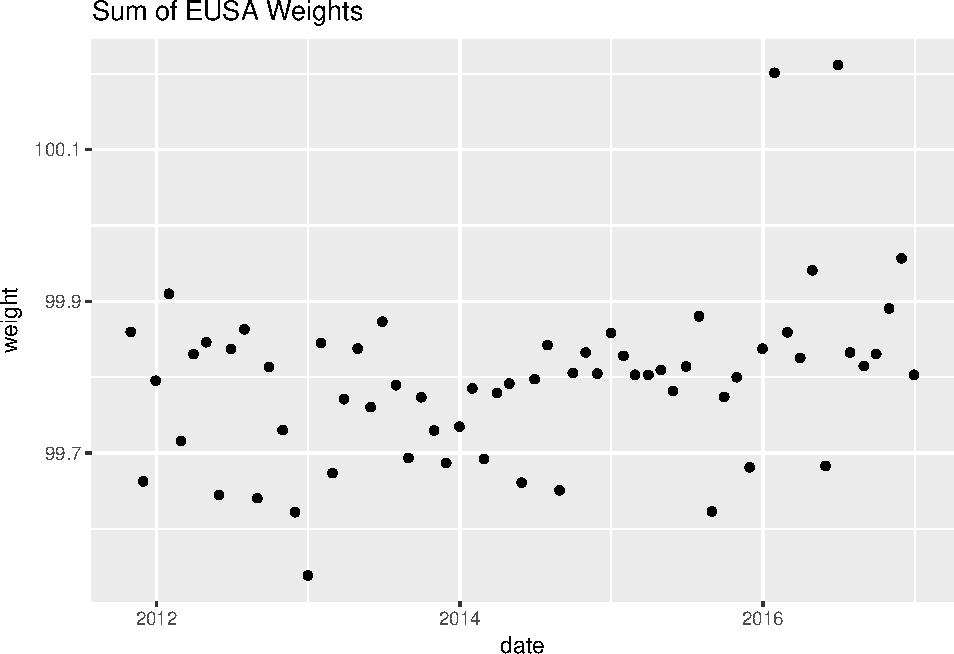
\includegraphics{thesis_files/figure-latex/unnamed-chunk-21-1.pdf} Shown
in the scatterplot above, the weights are very close to 100\%, with just
two months exceeding 100\%. The minimum weight is 99.54\%, while the
largest weight is 100.21\%. The mean weight is 99.79\%.

The monthly change in weights for the constructed Minimum Volatility
Index is shown below:
\begin{verbatim}
      date                weight     
 Min.   :2011-10-31   Min.   :99.58  
 1st Qu.:2013-02-14   1st Qu.:99.72  
 Median :2014-05-30   Median :99.76  
 Mean   :2014-05-30   Mean   :99.76  
 3rd Qu.:2015-09-15   3rd Qu.:99.81  
 Max.   :2016-12-30   Max.   :99.99  
\end{verbatim}
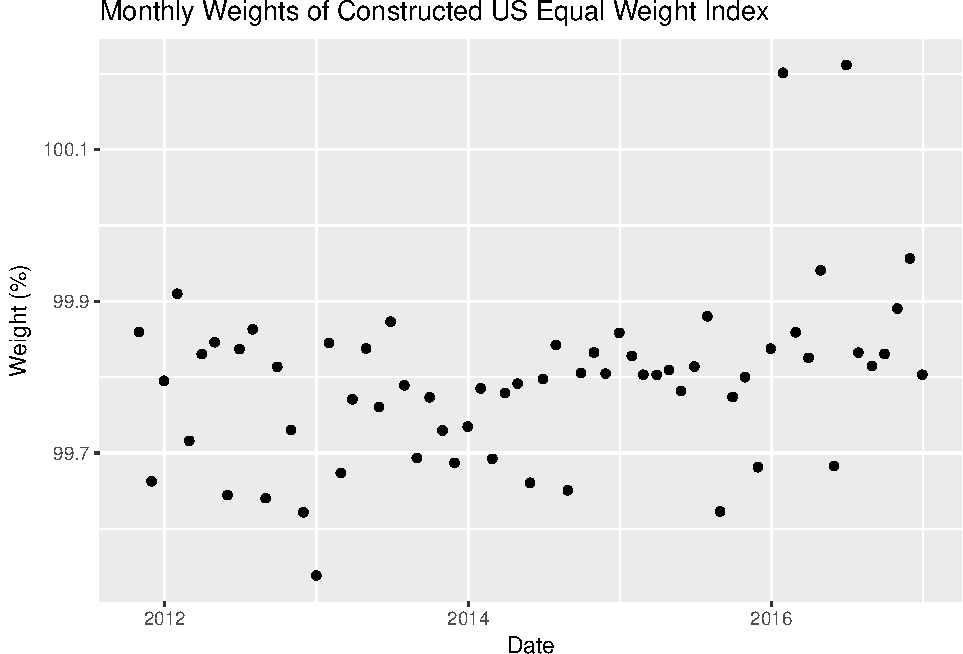
\includegraphics{thesis_files/figure-latex/unnamed-chunk-22-1.pdf} As
shown in the scatterplot above, the weights for USMV are very close to
100\%, with no value exceeding 100\%. The minimum weight is 99.58\%,
while the largest weight is 99.99\%. The mean weight is 99.76\%.

\subsection{Comparing Actual ETF returns to Constructed Index
returns}\label{comparing-actual-etf-returns-to-constructed-index-returns}

Given the weights were very close to 100\% for both ETFs on a monthly
basis, an additional check was performed by comparing the weighted
returns of the constructed indices to the actual ETFs that mirror them.
The ETFs are traded in the stock market, so price daily information on
each was widely available. Thus, this provided a way to check how the
constructed weighted returns compared to the ETF returns for both the
constructed US Equal Weight Index and Minimum Volatility Index.
Correlations were calculated between the performance of the constructed
US Equal Weight Index and EUSA, as well as between the performance of
the constructed Minimum Volatility Index and USMV.

For the Constructed US Equal Weight Index and EUSA:

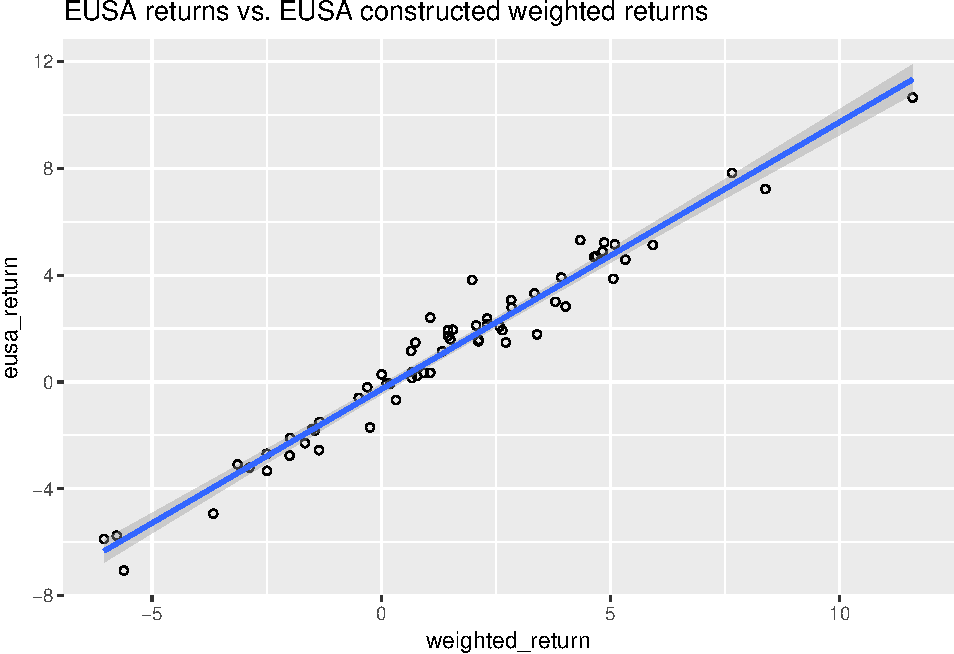
\includegraphics{thesis_files/figure-latex/unnamed-chunk-23-1.pdf}
\begin{verbatim}
                       [,1]
Delt.1.arithmetic 0.9805503
\end{verbatim}
The correlation between the Constructed US Equal Weight Index returns
and EUSA ETF returns, is 0.9805503.

For the Constructed Minimum Volatility Index and USMV:

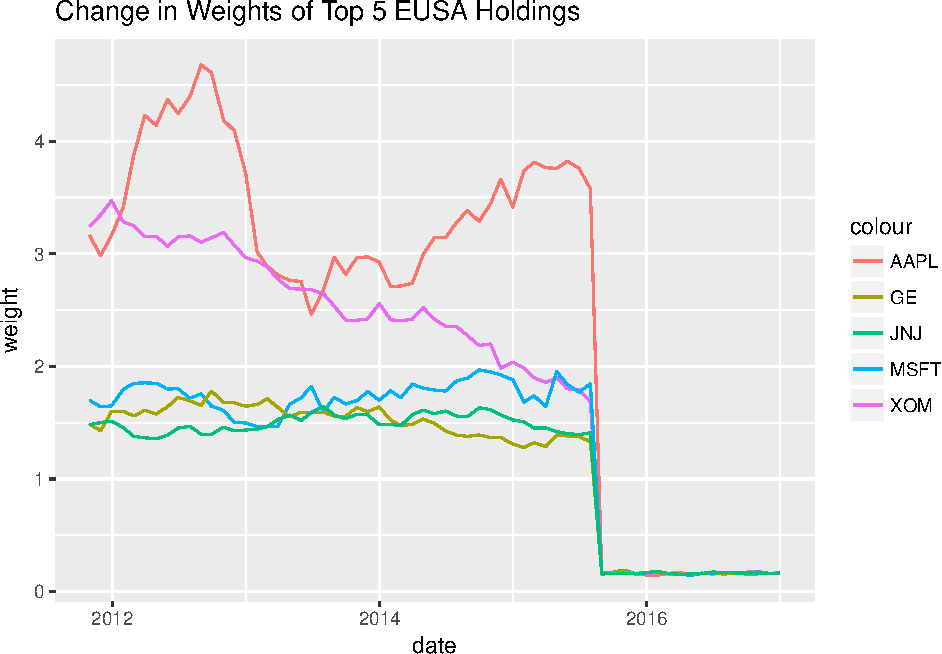
\includegraphics{thesis_files/figure-latex/unnamed-chunk-25-1.pdf}
\begin{verbatim}
                       [,1]
Delt.1.arithmetic 0.9906848
\end{verbatim}
The correlation is 0.99.

\subsection{Change in 5 largest holdings by average weight for EUSA and
USMV}\label{change-in-5-largest-holdings-by-average-weight-for-eusa-and-usmv}

The next thing we want to see is how the top 5 largest holdings, by
average weight, in each index have changed in weighting over time. For
EUSA, the 5 largest holdings were AAPL, XOM, MSFT, GE, and JNJ. Their
change in weights are shown below.
\begin{verbatim}
Warning in data(usa): data set 'usa' not found
\end{verbatim}
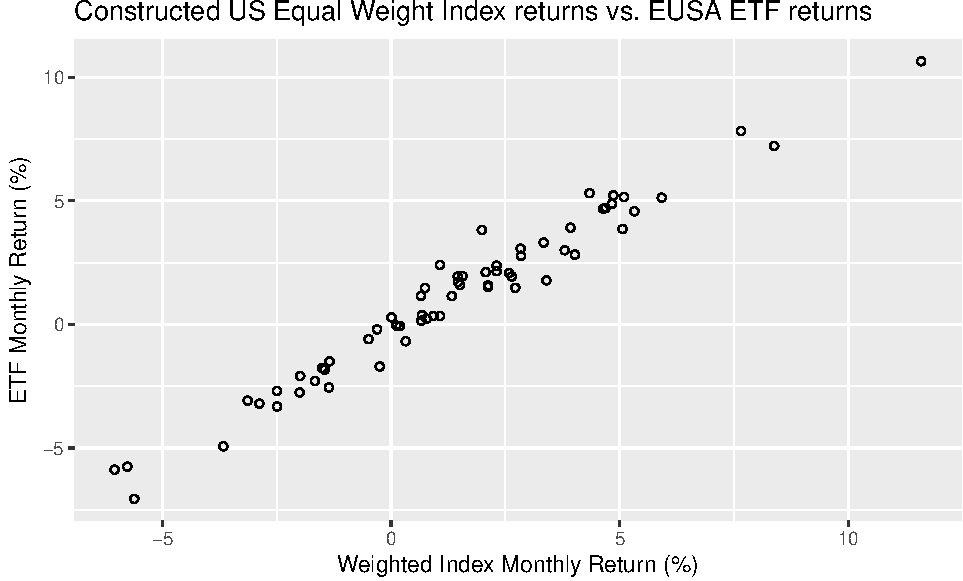
\includegraphics{thesis_files/figure-latex/unnamed-chunk-26-1.pdf}

Shown above, for EUSA, are some very interesting findings. The weights
of the 5 companies are all very high, then suddenly all spike. Verifying
this in the data, showed that for all 5 companies, holdings dropped
significantly between 2015-07-31 and 2015-08-31. The reason for this is
not entirely clear, but the general ETF started performing poorly around
this time too. In July of 2015 the price per share was 45.20, then it
dropped to 42.60 the following month, and dropped again to 40.50 in
August 2015. Perhaps these large companies were doing poorly, and MSCI
decided to try underweighting them.

For USMV, the 5 largest holdings were VZ, T, ADP, JNJ, and MCD. Their
change in weights are shown below. As we can see below, with the
exception of Verizon, the holdings generally remain between 1 and 1.6
percent of the overall portfolio.

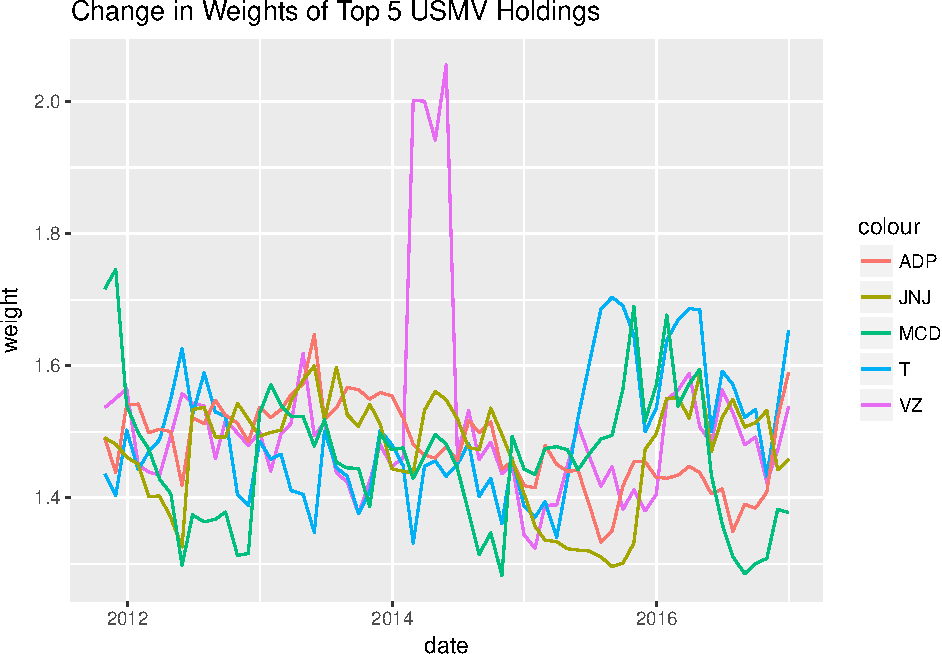
\includegraphics{thesis_files/figure-latex/unnamed-chunk-27-1.pdf}

\chapter{This chunk ensures that the thesisdown package
is}\label{this-chunk-ensures-that-the-thesisdown-package-is}

Placeholder

\section{Tables}\label{tables}

\section{Figures}\label{figures}

\section{Footnotes and Endnotes}\label{footnotes-and-endnotes}

\section{Bibliographies}\label{bibliographies}

\section{Anything else?}\label{anything-else}

\chapter*{Conclusion}\label{conclusion}
\addcontentsline{toc}{chapter}{Conclusion}

Placeholder

\chapter{The First Appendix}\label{the-first-appendix}

Placeholder

\chapter*{References}\label{references}
\addcontentsline{toc}{chapter}{References}

Placeholder

\hypertarget{refs}{}
\hypertarget{ref-blackrock2017}{}
BlackRock. (2017, September). IShares edge msci min vol usa etf
\textbar{} usmv. Retrieved from
\url{https://www.ishares.com/us/products/239695/ishares-msci-usa-minimum-volatility-etf}


% Index?

\end{document}
